% =====================================================================
\chapter{PHÂN TÍCH VÀ THIẾT KẾ HỆ THỐNG}\label{chap:thietke}
% =====================================================================

\section{Yêu cầu chức năng}\label{chap:usecase}
Yêu cầu chức năng được mô hình hóa bằng use case. Mỗi use case biểu diễn một mục tiêu có ý
nghĩa của một tác nhân và cho ra một kết quả quan sát được; các tình huống phụ như quẹt sai
cổng hay mất gói tin được xem là luồng ngoại lệ của use case chứa nó, không tách thành use case
riêng. Theo nguyên tắc này, hệ thống có 10 use case không chồng lấn nhau.

Hệ thống có hai tác nhân chính và bốn tác nhân phụ. Người lái xe là tác nhân chính của các use
case gửi xe, lấy xe và xem chỗ trống. Người vận hành là tác nhân chính của các use case quản lý
bãi thực hiện qua trang web. Sensor Client và RFID Client là hai tác nhân thiết bị cung cấp dữ
liệu cảm biến và sự kiện quẹt thẻ. Đồng hồ hệ thống là tác nhân thời gian kích hoạt việc đóng
thanh chắn và hết hạn chờ thanh toán. SePay là hệ thống bên ngoài cung cấp danh sách giao dịch
chuyển khoản vào tài khoản của bãi.

\begin{figure}[H]
\centering
\begin{tikzpicture}[
  uc/.style={draw=accent,fill=boxA,rounded corners=8pt,font=\footnotesize,align=center,text width=6.4cm,minimum height=0.74cm,inner sep=2pt},
  who/.style={draw,rounded corners=8pt,fill=white,font=\footnotesize,align=center,text width=2.6cm,minimum height=0.8cm,inner sep=2pt},
  dev/.style={draw,font=\footnotesize,align=center,text width=2.9cm,inner sep=3pt},
  link/.style={draw=black!65}]
\foreach \id/\txt [count=\i from 0] in {
  01/Xem chỗ trống tại cổng, 02/Gửi xe bằng thẻ RFID, 03/Thanh toán phí và lấy xe,
  06/Báo cháy và mở lối thoát, 07/Báo ngập và ngừng nhận xe, 08/Xem tình trạng bãi trên trang web,
  04/Xác nhận thanh toán tại quầy, 05/Điều khiển thanh chắn từ xa,
  09/Tra cứu nhật ký và doanh thu, 10/Hiệu chỉnh danh sách xe trong bãi}
  \node[uc] (UC\id) at (0,-\i*0.94) {UC\id\ \txt};
\begin{scope}[on background layer]
  \node[fill=boxC,draw=black!25,fit=(UC01)(UC10),inner xsep=6pt,inner ysep=6pt,
        label={[font=\footnotesize\bfseries,anchor=south]north:Hệ thống bãi đỗ xe thông minh}] {};
\end{scope}
\node[who] (driver) at (-6.7,-1.4) {Người lái xe};
\node[who] (oper) at (-6.7,-6.1) {Người vận hành};
\node[dev,fill=boxB] (sensor) at (6.75,-3.3) {«thiết bị»\\Sensor Client};
\node[dev,fill=boxC] (rfid) at (6.75,-0.9) {«thiết bị»\\RFID Client};
\node[dev,fill=boxE] (clock) at (6.75,-5.4) {«thời gian»\\Đồng hồ hệ thống};
\node[dev,fill=boxE] (sepay) at (6.75,-7.4) {«hệ thống ngoài»\\SePay};
\foreach \u in {01,02,03,06} \draw[link] (driver.east) -- (UC\u.west);
\foreach \u in {06,07,08,04,05,09,10} \draw[link] (oper.east) -- (UC\u.west);
\foreach \u in {01,06,07,08} \draw[link] (UC\u.east) -- (sensor.west);
\foreach \u in {02,03,08} \draw[link] (UC\u.east) -- (rfid.west);
\foreach \u in {02,03} \draw[link,densely dashed] (UC\u.east) -- (clock.west);
\draw[link] (UC03.east) -- (sepay.west);
\end{tikzpicture}
\caption{Sơ đồ use case tổng quát}\label{fig:usecase}
\end{figure}

Hình~\ref{fig:usecase} thể hiện quan hệ giữa các tác nhân và 10 use case. Ba use case đầu phục
vụ người lái xe trong một lượt gửi xe trọn vẹn; hai use case tiếp theo là phản ứng tự động của hệ
thống trước sự cố, có cả người lái và người vận hành tham gia; năm use case còn lại là nghiệp vụ
của người vận hành trên trang web. Đường nét đứt biểu diễn sự kiện theo thời gian như đóng thanh
chắn hay hết hạn chờ thanh toán. Bảng~\ref{tab:uc-summary} tóm tắt tác nhân chính và mục tiêu của
từng use case; đặc tả đầy đủ và cách hiện thực được trình bày theo đúng thứ tự này ở
Chương~\ref{chap:hienthuc}.

\begin{table}[H]
\centering\small
\caption{Tổng hợp các use case}\label{tab:uc-summary}
\begin{tabularx}{\linewidth}{@{}l>{\raggedright\arraybackslash}p{4.3cm}>{\raggedright\arraybackslash}p{2.6cm}X@{}}
\toprule
Mã & Tên use case & Tác nhân chính & Mục tiêu \\ \midrule
UC01 & Xem chỗ trống tại cổng & Người lái xe & Biết bãi còn bao nhiêu chỗ và chỗ nào trống trước khi vào \\
UC02 & Gửi xe bằng thẻ RFID & Người lái xe & Được mở cổng vào và bắt đầu tính thời gian gửi xe \\
UC03 & Thanh toán phí và lấy xe & Người lái xe & Trả đúng phí bằng VietQR và được mở cổng ra \\
UC04 & Xác nhận thanh toán tại quầy & Người vận hành & Cho xe ra khi khách trả tiền mặt hoặc không đối soát tự động được \\
UC05 & Điều khiển thanh chắn từ xa & Người vận hành & Mở hoặc đóng từng cổng hay cả hai cổng khi cần \\
UC06 & Báo cháy và mở lối thoát & Sensor Client & Báo động và giải phóng lối ra ngay khi có lửa \\
UC07 & Báo ngập và ngừng nhận xe & Sensor Client & Báo động và không cho thêm xe vào khi nước dâng \\
UC08 & Xem tình trạng bãi trên trang web & Người vận hành & Nắm được trạng thái ô đỗ, môi trường và thanh chắn từ xa \\
UC09 & Tra cứu nhật ký và doanh thu & Người vận hành & Đối soát lượt xe vào ra và tiền thu được \\
UC10 & Hiệu chỉnh danh sách xe trong bãi & Người vận hành & Xóa xe đã rời bãi mà không qua quy trình ra bình thường \\
\bottomrule
\end{tabularx}
\end{table}

\section{Yêu cầu phi chức năng}\label{sec:nfr}
Bên cạnh chức năng, hệ thống phải đáp ứng các yêu cầu về thời gian, an toàn, độ tin cậy và
tài nguyên. Bảng~\ref{tab:nfr} lượng hóa từng yêu cầu và nêu giải pháp thiết kế tương ứng.

\begin{table}[H]
\centering\small
\caption{Yêu cầu phi chức năng và giải pháp đáp ứng}\label{tab:nfr}
\begin{tabularx}{\linewidth}{@{}p{2.6cm}X>{\raggedright\arraybackslash}p{5cm}@{}}
\toprule
Yêu cầu & Chỉ tiêu & Giải pháp thiết kế \\ \midrule
Thời gian đáp ứng & Màn hình cập nhật dưới 0,2\,s sau khi xe vào ô; thanh chắn mở dưới 0,5\,s sau khi quẹt thẻ & Gửi dữ liệu khi có thay đổi, vẽ màn hình theo sự kiện, tác vụ mạng có ưu tiên cao \\
An toàn & Có cháy thì mở cả hai cổng ngay; không hạ thanh chắn khi xe còn trong cổng; có ngập thì không nhận xe & Chế độ cháy ưu tiên cao nhất; cảm biến IR tại cổng; chặn quẹt thẻ vào khi ngập \\
Độ tin cậy & Không mất lượt quẹt thẻ khi mất gói; không mất dữ liệu gửi xe khi mất điện & Xác nhận và gửi lại; lưu phiên vào bộ nhớ flash \\
Tài nguyên & Chạy trong khoảng 321\,KB RAM cùng ảnh màn hình 115\,KB và kết nối TLS & Cấp phát bộ đệm TLS động, giải phóng bộ đệm ảnh động khi thanh toán \\
Bảo mật & Thao tác điều khiển cần xác thực; thông tin bí mật không nằm trong mã nguồn & Mã PIN quản trị; cấu hình bí mật qua menuconfig \\
Dễ sử dụng & Dùng được trên mọi điện thoại, thanh toán bằng ứng dụng ngân hàng bất kỳ & Trang web tại \code{parking.local}, mã VietQR \\
\bottomrule
\end{tabularx}
\end{table}

Các chỉ tiêu trong Bảng~\ref{tab:nfr} chi phối nhiều quyết định thiết kế ở các mục sau. Yêu
cầu thời gian dẫn tới việc gửi dữ liệu theo sự kiện thay vì theo chu kỳ; yêu cầu an toàn dẫn
tới việc bổ sung cảm biến hồng ngoại dưới mỗi thanh chắn; yêu cầu tài nguyên buộc máy chủ
phải quản lý bộ nhớ động một cách có chủ đích khi thực hiện kết nối HTTPS.

\section{Kiến trúc tổng thể}\label{sec:trienkhai}
Hệ thống gồm ba thiết bị cùng kết nối vào một mạng Wi-Fi chung có Internet. Hình~\ref{fig:deploy}
mô tả kiến trúc triển khai và luồng dữ liệu giữa các thành phần.

\begin{figure}[H]
\centering
\mmd[0.95][0.55]{deploy}
\caption{Kiến trúc triển khai và luồng dữ liệu}\label{fig:deploy}
\end{figure}

Theo Hình~\ref{fig:deploy}, mạng có cấu trúc hình sao quanh router; cả ba thiết bị và điện
thoại của người vận hành đều kết nối tới router như các thiết bị Wi-Fi thông thường, nên thứ
tự bật nguồn không quan trọng. Sensor Client và RFID Client gửi gói UDP tới địa chỉ quảng bá
\code{255.255.255.255}, cổng 3333, nên không cần biết dải mạng hay địa chỉ IP của máy chủ.
Người vận hành truy cập máy chủ bằng tên cố định \code{parking.local}; máy chủ chủ động thông
báo lại tên này mỗi khi được cấp địa chỉ mới, nên tên luôn trỏ đúng thiết bị dù DHCP thay đổi
địa chỉ. Router đồng thời là đường ra Internet để máy chủ truy vấn giao dịch trên SePay.

Kiến trúc tách thành ba thiết bị mang lại hai lợi ích: đặt cảm biến gần nơi cần đo để dây
ngắn, và cô lập lỗi khi một thiết bị mất điện. Đổi lại, hệ thống phụ thuộc vào mạng Wi-Fi;
Mục~\ref{sec:uc08} trình bày cách máy chủ phát hiện client mất kết nối.

\section{Thiết kế phần cứng}\label{sec:phancung}
\subsection{Thuyết minh mạch điện}\label{sec:schematic}
Mạch điện của hệ thống gồm ba bản vẽ, mỗi bản vẽ ứng với một thiết bị và có đầu vào nguồn
5\,V riêng. Trước khi đi vào từng bản vẽ, Hình~\ref{fig:power} tóm tắt đường đi của nguồn
điện, phần quyết định độ ổn định của toàn hệ thống.

\begin{figure}[H]
\centering
\begin{tikzpicture}[
  blk/.style={draw,rounded corners=2pt,font=\footnotesize,align=center,minimum height=0.95cm,inner sep=3pt},
  ld/.style={blk,fill=boxB,text width=2.6cm},
  arr/.style={-{Stealth[length=2mm]},thick},
  v/.style={font=\scriptsize\itshape,text=accent}]
% Server
\node[font=\footnotesize\bfseries,anchor=west] at (-0.2,1.15) {Máy chủ};
\node[blk,fill=boxC] (a1) at (1,0) {Adapter\\5\,V};
\node[blk,fill=boxA] (c1) at (3.3,0) {C1 100\,µF\\lọc đầu vào};
\node[ld] (sv) at (7,0.75) {2 servo SG90\\C2, C3 100\,µF};
\node[blk,fill=boxA] (u1) at (7,-0.75) {C4 10\,µF + ổn áp\\trên ESP32-C3};
\node[ld] (l3) at (11.3,-0.75) {TFT, còi,\\2 IR cổng};
\draw[arr] (a1) -- (c1);
\draw[arr] (c1.east) -- ++(0.5,0) |- node[v,above,pos=0.75] {5\,V} (sv.west);
\draw[arr] (c1.east) -- ++(0.5,0) |- node[v,below,pos=0.75] {5\,V} (u1.west);
\draw[arr] (u1) -- node[v,above] {3,3\,V} (l3);
% Client
\node[font=\footnotesize\bfseries,anchor=west] at (-0.2,-2.25) {Mỗi client};
\node[blk,fill=boxC] (a2) at (1,-3.4) {Adapter\\5\,V};
\node[blk,fill=boxA] (c5) at (3.3,-3.4) {C5 hoặc C6\\100\,µF};
\node[blk,fill=boxD] (d1) at (5.7,-3.4) {Diode\\1N4007};
\node[blk,fill=boxD] (d2) at (7.9,-3.4) {Diode\\1N4007};
\node[ld] (l2) at (11.6,-3.4) {ESP8266 và\\toàn bộ cảm biến};
\draw[arr] (a2) -- (c5); \draw[arr] (c5) -- node[v,above] {5\,V} (d1);
\draw[arr] (d1) -- node[v,above] {4,3\,V} (d2); \draw[arr] (d2) -- node[v,above] {3,6\,V} (l2);
\end{tikzpicture}
\caption{Đường cấp nguồn của máy chủ và của mỗi client}\label{fig:power}
\end{figure}

Hình~\ref{fig:power} cho thấy hai cách cấp nguồn khác nhau. Máy chủ có hai nhánh: nhánh 5\,V
cấp trực tiếp cho servo, nhánh còn lại đi qua bộ ổn áp 3,3\,V có sẵn trên bo ESP32-C3 SuperMini
để cấp cho màn hình, còi và hai cảm biến cổng. Mỗi client hạ 5\,V xuống khoảng 3,6\,V bằng hai
diode mắc nối tiếp rồi cấp chung cho ESP8266 và các cảm biến. Ba bản vẽ chi tiết ở
Hình~\ref{fig:sch-server}, \ref{fig:sch-sensor} và \ref{fig:sch-rfid} được thuyết minh lần
lượt trong ba mục sau.

\subsubsection{Mạch máy chủ}
\begin{sidewaysfigure}
\centering
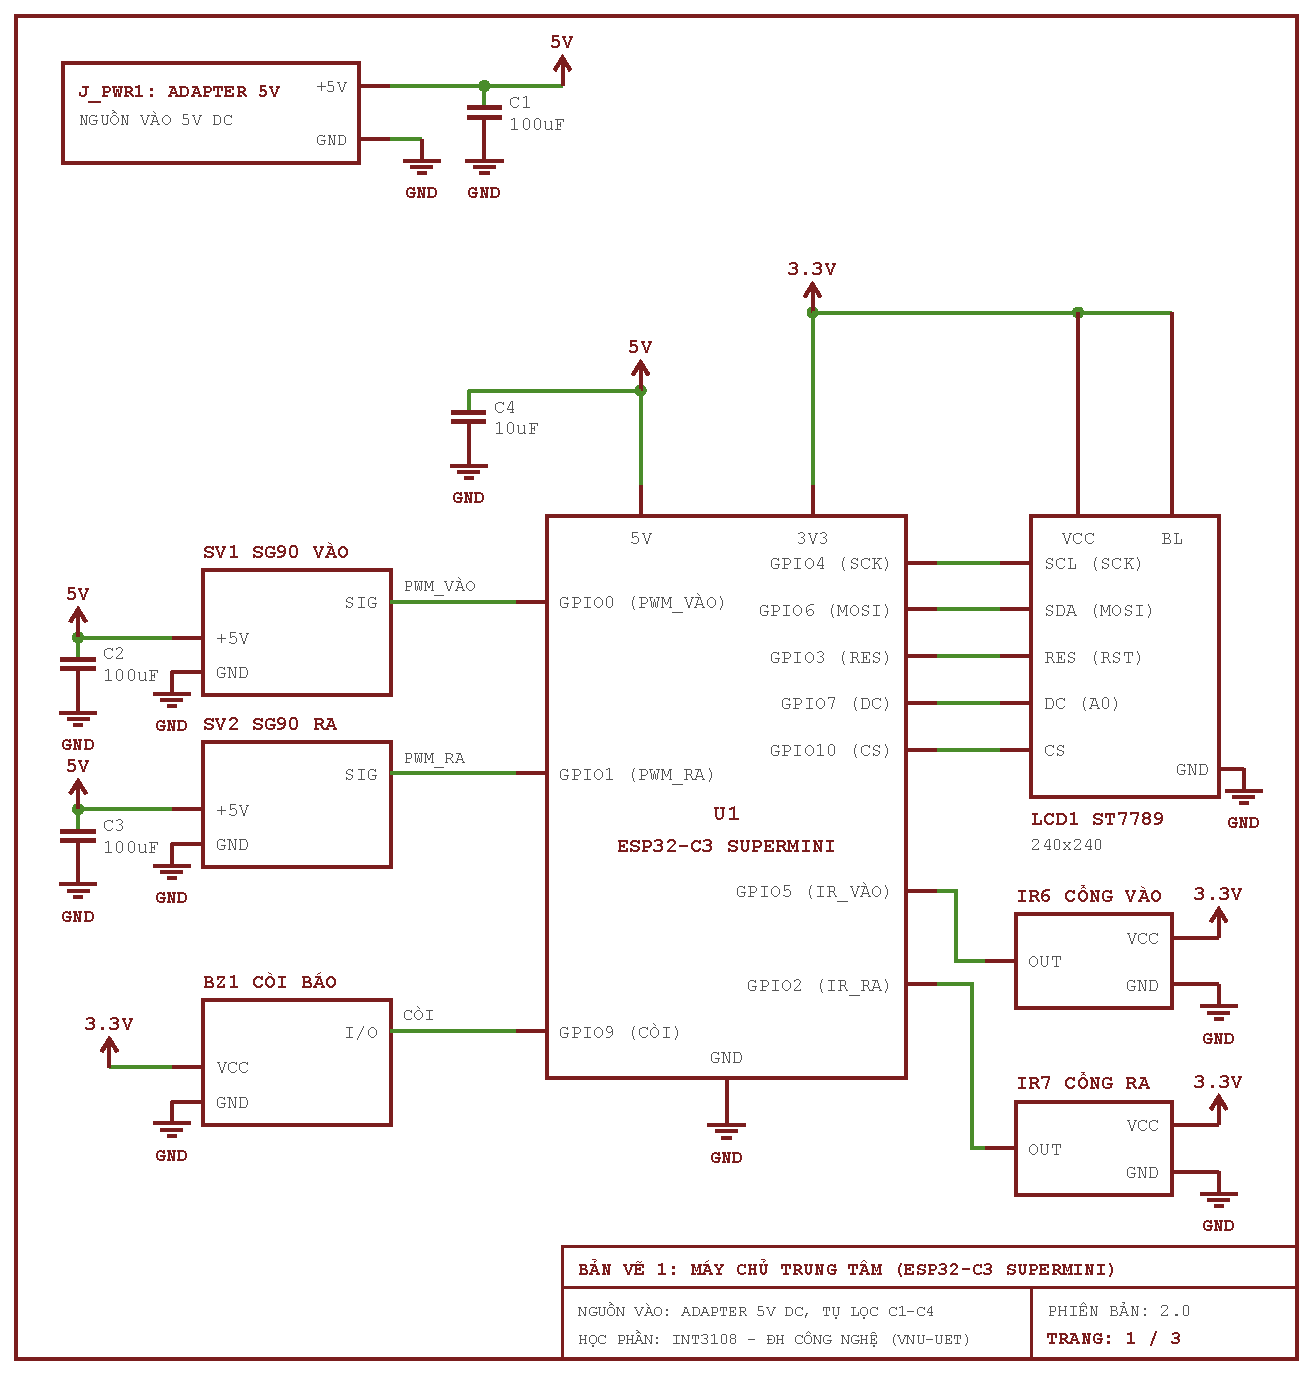
\includegraphics[width=\linewidth,height=0.82\textwidth,keepaspectratio]{schematic/sheet1.pdf}
\caption{Sơ đồ nguyên lý máy chủ: ESP32-C3, màn hình ST7789, 2 servo, còi và 2 cảm biến IR ở cổng}\label{fig:sch-server}
\end{sidewaysfigure}

Hình~\ref{fig:sch-server} là mạch máy chủ. Adapter J\_PWR1 cấp đường 5\,V chung; tụ hóa C1
100\,µF đặt ngay đầu vào san phẳng gợn sóng của adapter. Hai servo SG90 lấy nguồn trực tiếp từ đường 5\,V thay vì từ chân 3V3 của bo, vì
SG90 cần 4,8--6\,V và kéo dòng vài trăm mA lúc bắt đầu quay, vượt khả năng của bộ ổn áp nhỏ
trên bo. Mỗi servo có một tụ 100\,µF riêng (C2, C3) đặt sát chân nguồn. Khi động cơ khởi
động, dòng tức thời tăng vọt; nếu không có tụ, điện áp đường 5\,V sụt xuống và có thể làm
ESP32-C3 tự khởi động lại. Tụ cấp phần dòng tức thời này tại chỗ, đặc biệt cần thiết khi cả
hai servo quay cùng lúc trong chế độ cháy. Chân GND của adapter phải nối chung với GND của
ESP32-C3 để xung PWM trên GPIO0 và GPIO1 có cùng mức tham chiếu với servo.

Tụ C4 10\,µF đặt sát chân 5V của ESP32-C3 lọc nhiễu tần số cao và giữ ổn định điện áp vào bộ
ổn áp 3,3\,V trên bo trong các đợt phát Wi-Fi công suất cao. Đầu ra 3V3 của bo cấp cho màn
hình, còi và hai cảm biến hồng ngoại ở cổng. Ngõ ra của hai cảm biến cổng nối vào GPIO5
(cổng vào) và GPIO2 (cổng ra) với điện trở kéo lên nội được bật trong firmware. Còi nối vào
GPIO9 và được firmware đặt ở mức cao ngay khi khởi tạo để còi im lặng. Màn hình ST7789 nối qua
SPI2 với năm tín hiệu SCK, MOSI, RES, DC và CS; chân đèn nền BL nối thẳng lên 3,3\,V nên màn
hình luôn sáng.

\subsubsection{Mạch Sensor Client}
\begin{sidewaysfigure}
\centering
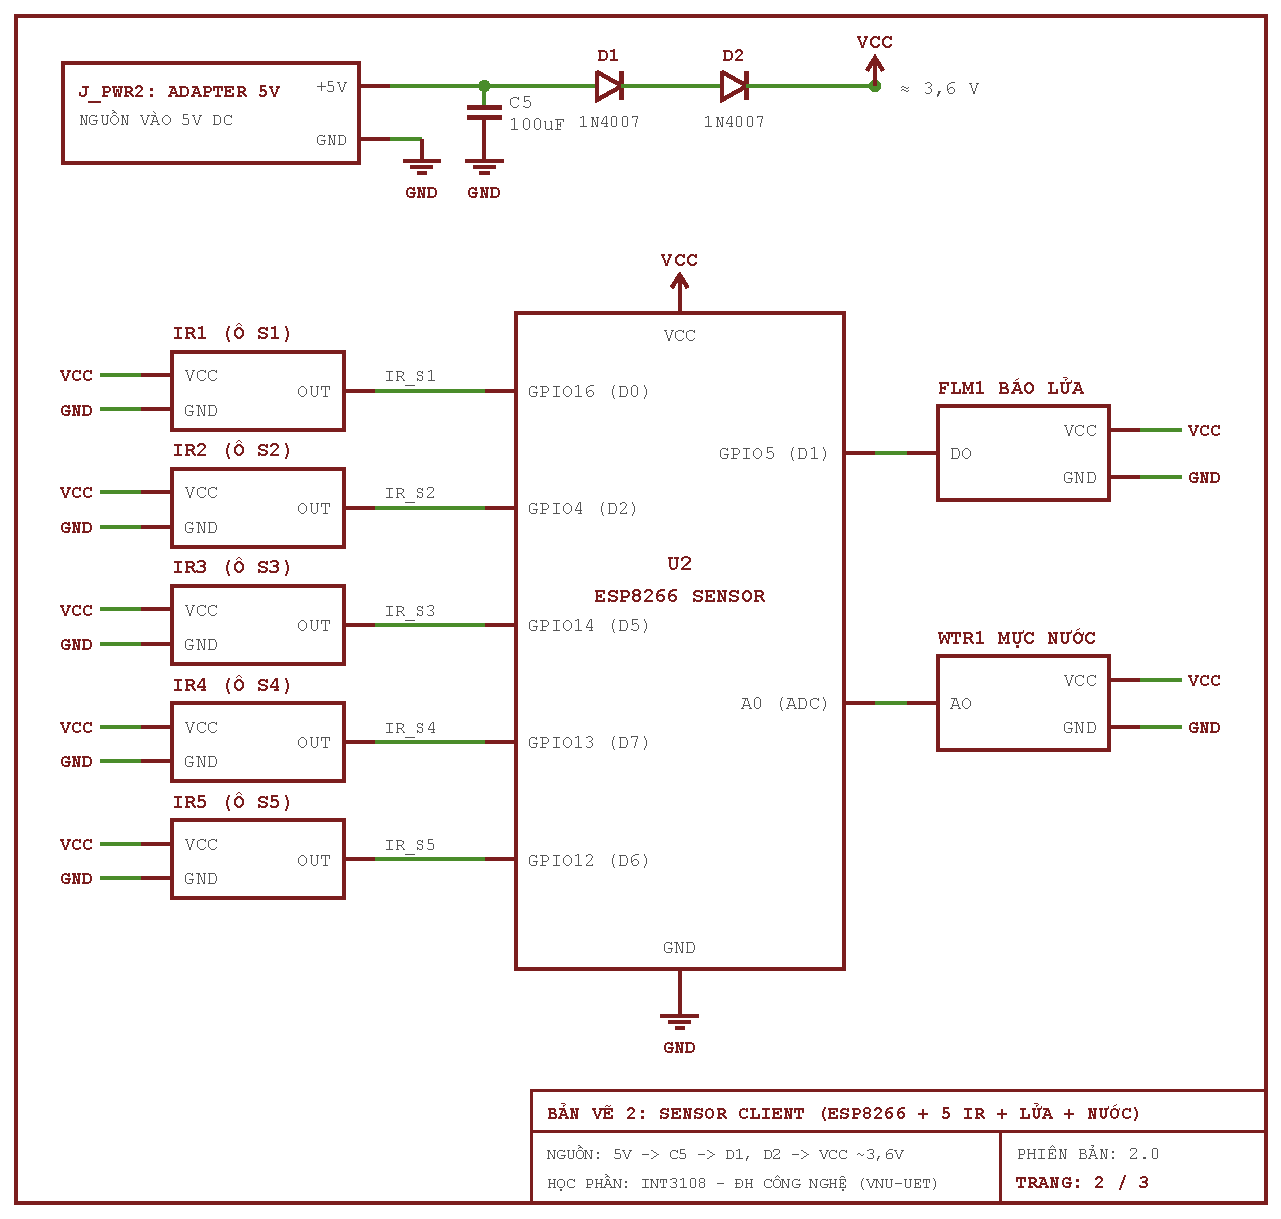
\includegraphics[width=\linewidth,height=0.82\textwidth,keepaspectratio]{schematic/sheet2.pdf}
\caption{Sơ đồ nguyên lý Sensor Client: ESP8266, 5 cảm biến IR ô đỗ, cảm biến lửa và mực nước}\label{fig:sch-sensor}
\end{sidewaysfigure}

Hình~\ref{fig:sch-sensor} là mạch Sensor Client. Adapter J\_PWR2 cấp 5\,V qua tụ C5 100\,µF,
sau đó qua hai diode chỉnh lưu 1N4007 (D1, D2) mắc nối tiếp để tạo đường VCC khoảng 3,6\,V cấp
chung cho module ESP8266 và các cảm biến. Mỗi diode silic có điện áp rơi thuận khoảng 0,7\,V
khi dẫn, nên điện áp sau hai diode là
\begin{equation}
  V_{CC} \approx V_{in} - 2V_F = 5 - 2\times0{,}7 = 3{,}6\ \text{V},
\end{equation}
nằm trong dải 3,0--3,6\,V của ESP8266. Cặp diode đảm nhiệm hai chức năng cùng lúc. Chức năng
thứ nhất là hạ áp mà không cần IC ổn áp, phù hợp với linh kiện sẵn có và dòng tiêu thụ nhỏ
của client. Chức năng thứ hai là bảo vệ ngược cực: nếu adapter bị cắm ngược, diode phân cực
ngược và chặn dòng, bảo vệ ESP8266 cùng các module. Công suất tiêu tán trên mỗi diode là
$P = V_F \cdot I \approx 0{,}7 \times 0{,}3 \approx 0{,}2$\,W ở đỉnh dòng khi phát Wi-Fi,
thấp hơn nhiều so với định mức 1\,A của 1N4007. Hạn chế của phương án là $V_F$ thay đổi theo
dòng tải, nên điện áp VCC dao động quanh 3,6\,V; tụ C5 phía trước giữ ổn định đầu vào.

Năm cảm biến hồng ngoại IR1 đến IR5 cùng lấy nguồn từ đường VCC, ngõ ra OUT nối lần lượt vào
GPIO16, 4, 14, 13 và 12. Vì cảm biến dùng chung nguồn với ESP8266, mức cao ở ngõ ra không vượt
quá điện áp chịu đựng của chân vào. Cảm biến lửa FLM1 nối ngõ ra digital DO vào GPIO5, cảm biến mực
nước WTR1 nối ngõ ra analog AO vào chân ADC A0.

\subsubsection{Mạch RFID Client}
\begin{sidewaysfigure}
\centering
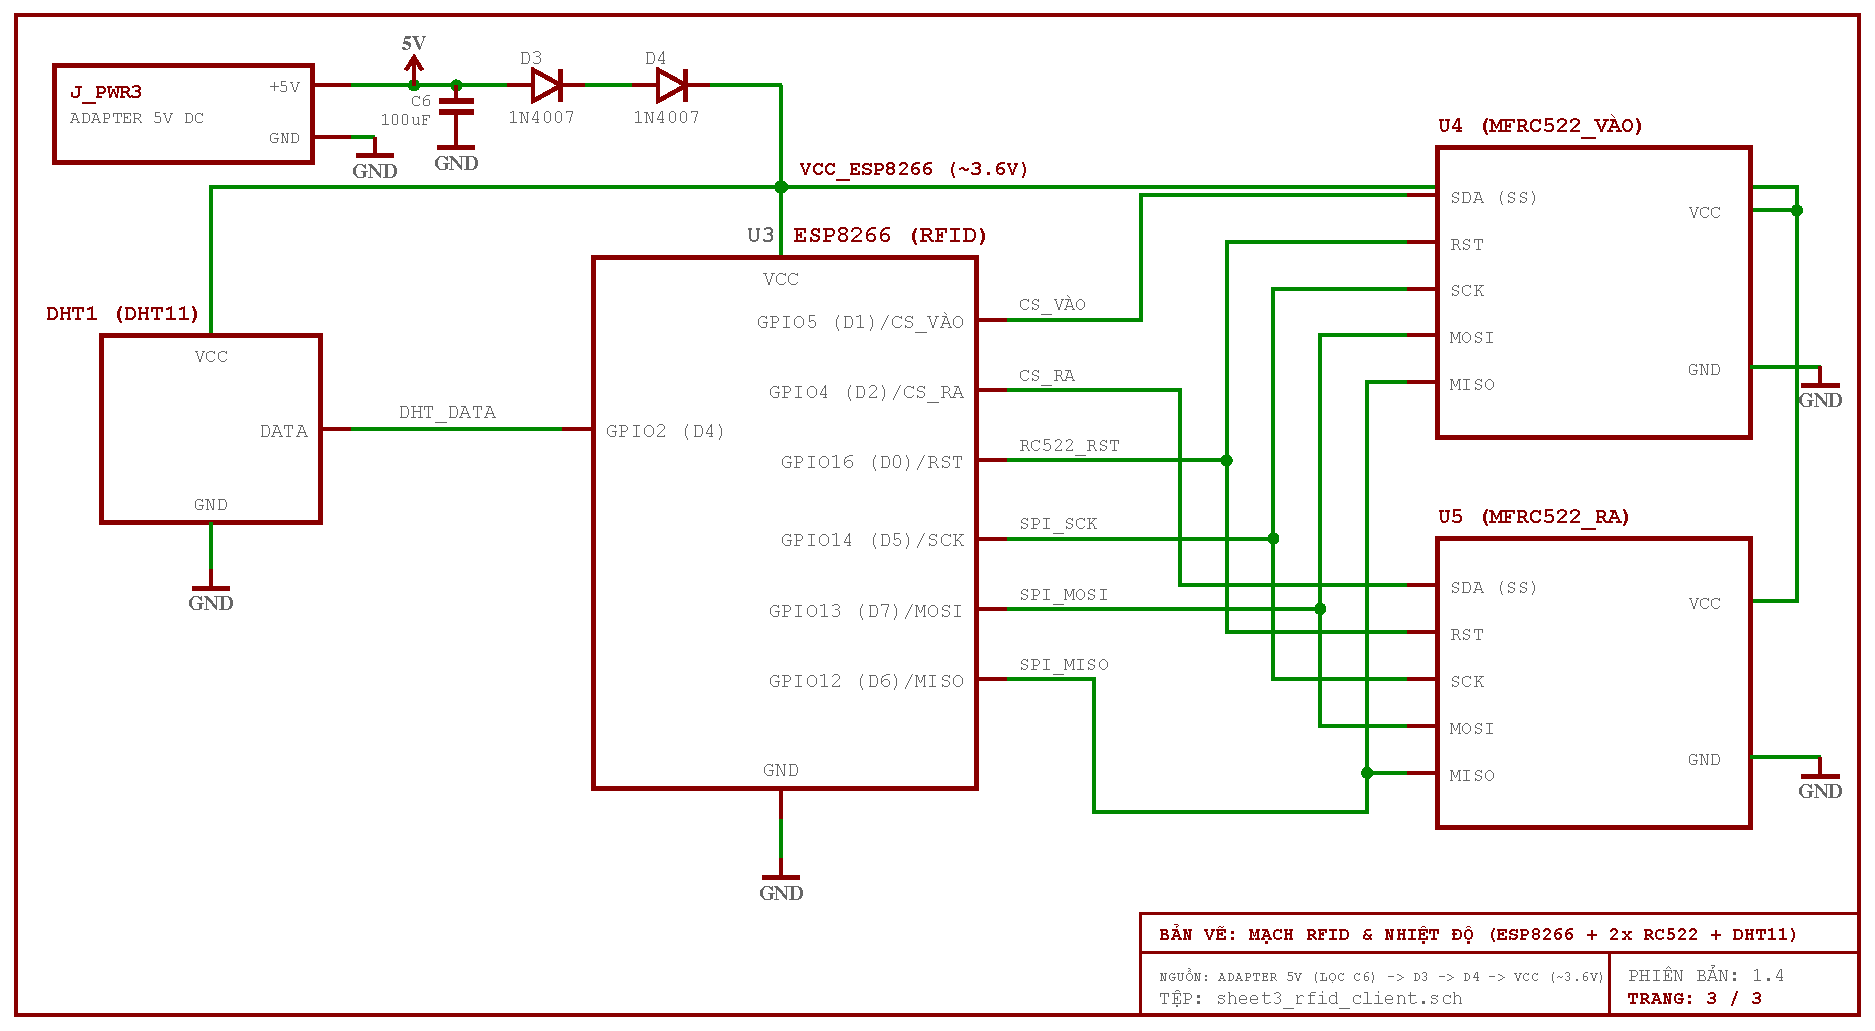
\includegraphics[width=\linewidth,height=0.82\textwidth,keepaspectratio]{schematic/sheet3.pdf}
\caption{Sơ đồ nguyên lý RFID Client: ESP8266, 2 đầu đọc RC522 dùng chung SPI và DHT11}\label{fig:sch-rfid}
\end{sidewaysfigure}

Hình~\ref{fig:sch-rfid} là mạch RFID Client, có đường nguồn giống Sensor Client gồm adapter
J\_PWR3, tụ C6 100\,µF và hai diode D3, D4. Tụ C6 có thêm vai trò ổn định điện áp khi hai
ăng-ten RC522 đóng cắt trường từ 13,56\,MHz và khi ESP8266 phát gói tin. Hai đầu đọc U4 (cổng
vào) và U5 (cổng ra) dùng chung bus SPI gồm SCK, MOSI, MISO ở GPIO14, 13, 12 và chân reset ở
GPIO16; mỗi đầu đọc có chân chọn chip SDA riêng là GPIO5 và GPIO4, nên tại mỗi thời điểm chỉ
một đầu đọc giao tiếp trên bus. Cảm biến DHT11 nối chân DATA vào GPIO2; đây là chân strapping
của ESP8266, cần mức cao khi khởi động, và điện trở kéo lên sẵn có trên module DHT11 bảo đảm
điều kiện này.

\subsection{Bố trí thiết bị trên mô hình}\label{sec:mohinh}
Mô hình được làm bằng bìa formex trắng, vật liệu nhẹ, cách điện và dễ khoét lỗ cho cảm biến.
Hình~\ref{fig:hw-photos} cho thấy ba khu vực lắp thiết bị chính ngoài hộp điều khiển đã giới
thiệu ở Hình~\ref{fig:overview}.

\begin{figure}[H]
\centering
\begin{subfigure}[t]{0.56\linewidth}\centering
  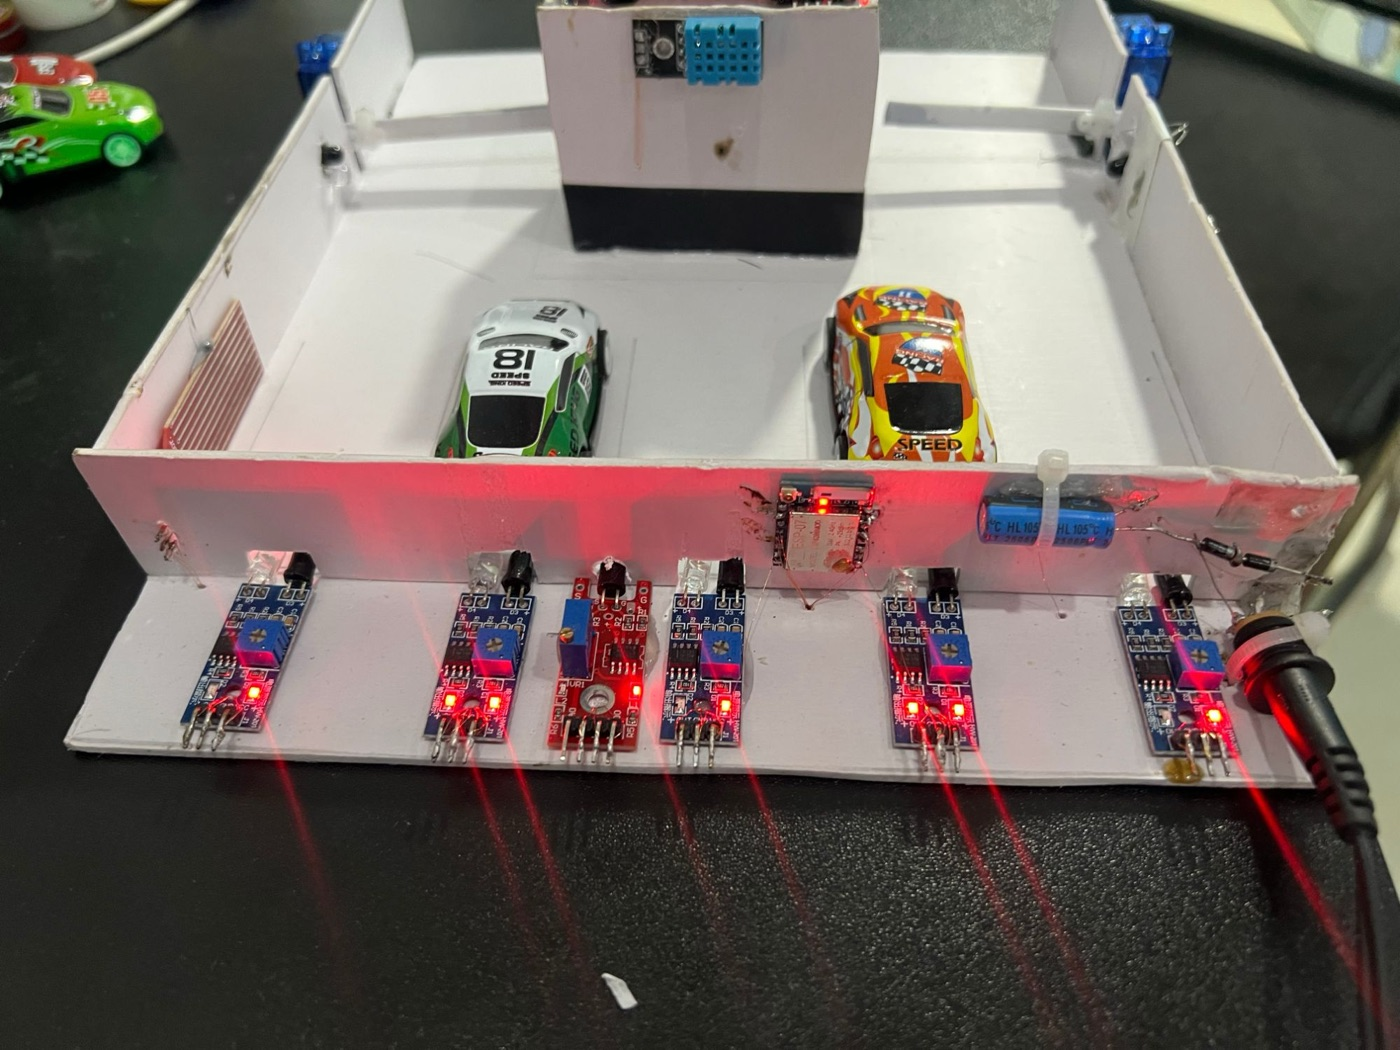
\includegraphics[width=\linewidth,height=0.3\textheight,keepaspectratio]{photos/model_back.jpg}
  \caption{Mặt ngoài vách sau: Sensor Client với 5 module IR, module lửa, mạch nguồn}\label{fig:model-back}
\end{subfigure}\hfill
\begin{subfigure}[t]{0.4\linewidth}\centering
  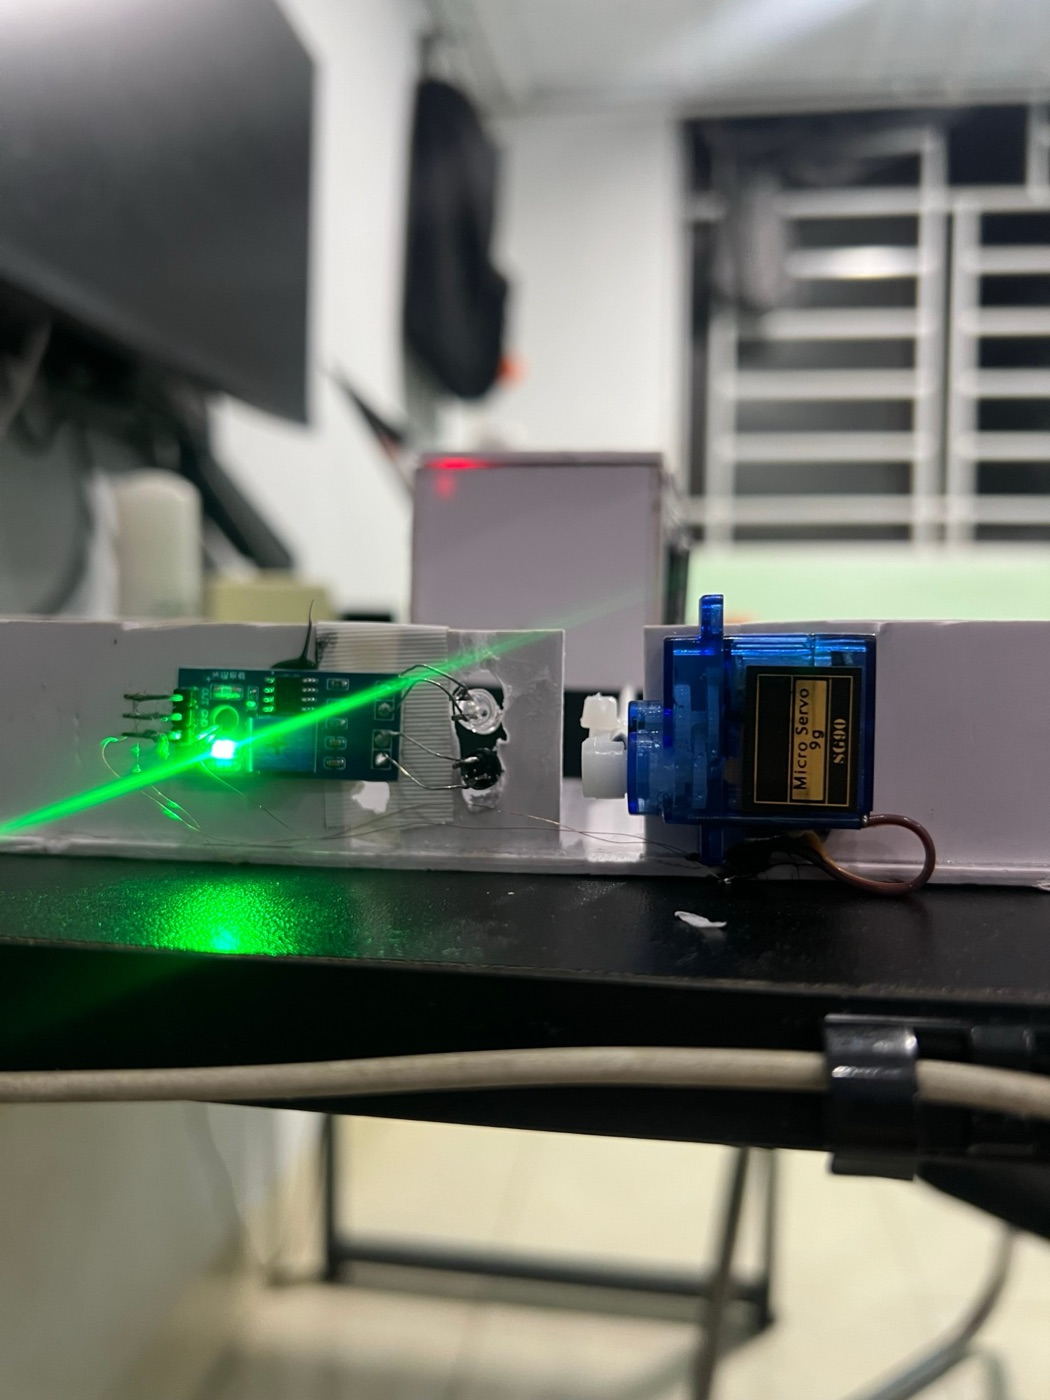
\includegraphics[width=\linewidth,height=0.3\textheight,keepaspectratio]{photos/gate_ir.jpg}
  \caption{Cổng ra: servo SG90 và module IR phát hiện xe trong cổng}\label{fig:gate-ir}
\end{subfigure}

\vspace{4pt}
\begin{subfigure}[t]{0.42\linewidth}\centering
  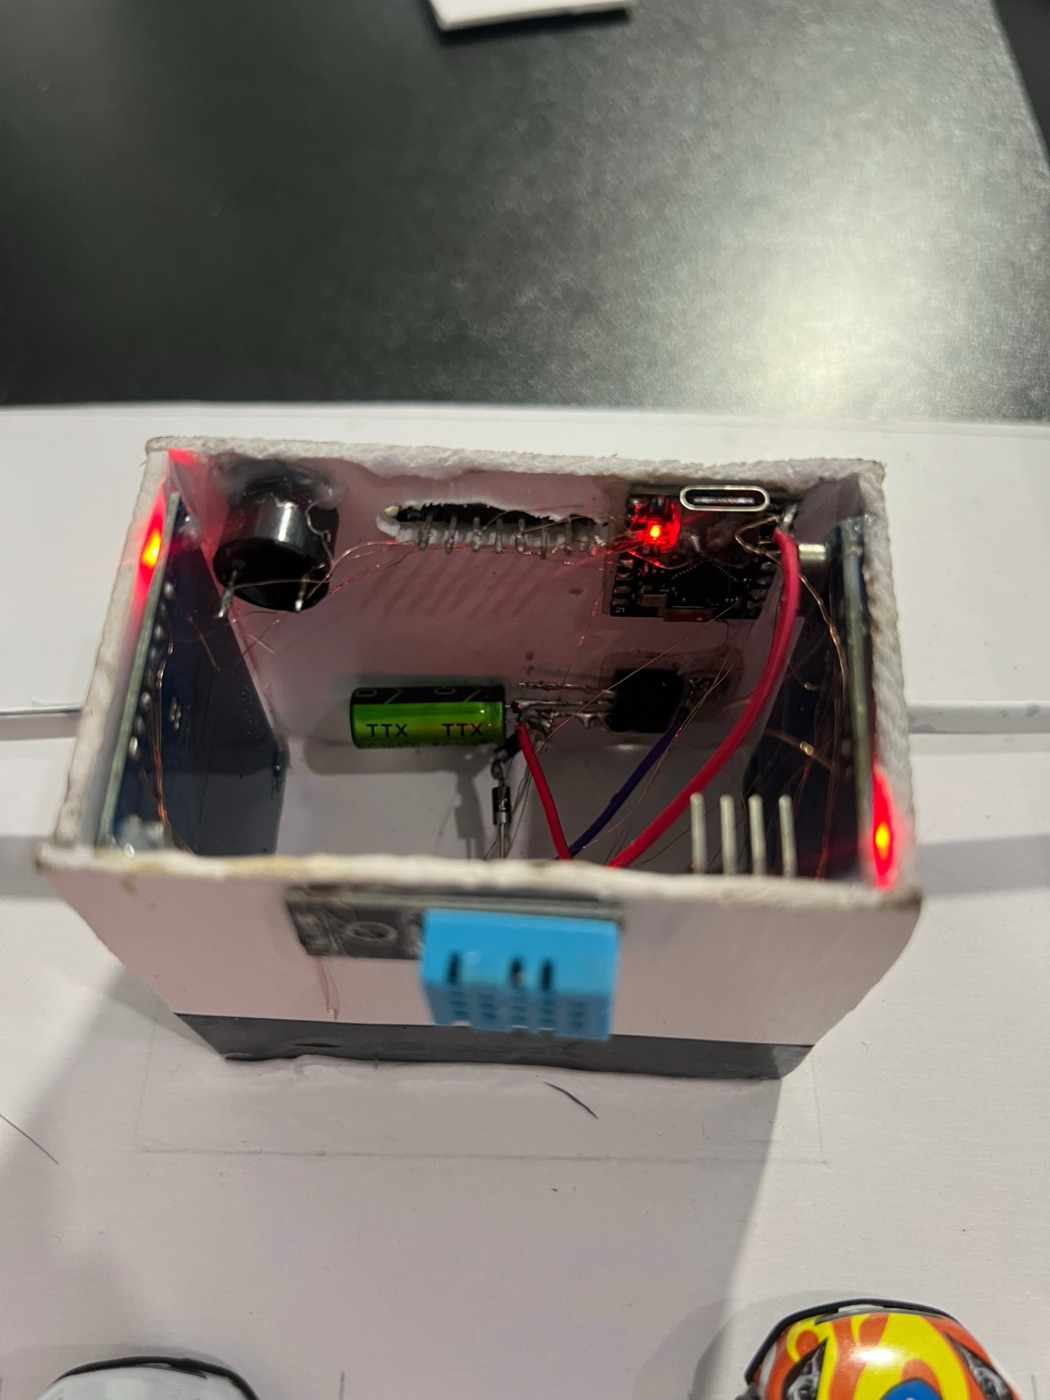
\includegraphics[width=\linewidth,height=0.3\textheight,keepaspectratio]{photos/box_inside.jpg}
  \caption{Bên trong hộp điều khiển: ESP32-C3, còi, mạch nguồn, hai đầu đọc RC522 ở hai thành hộp}\label{fig:box}
\end{subfigure}\hfill
\begin{subfigure}[t]{0.42\linewidth}\centering
  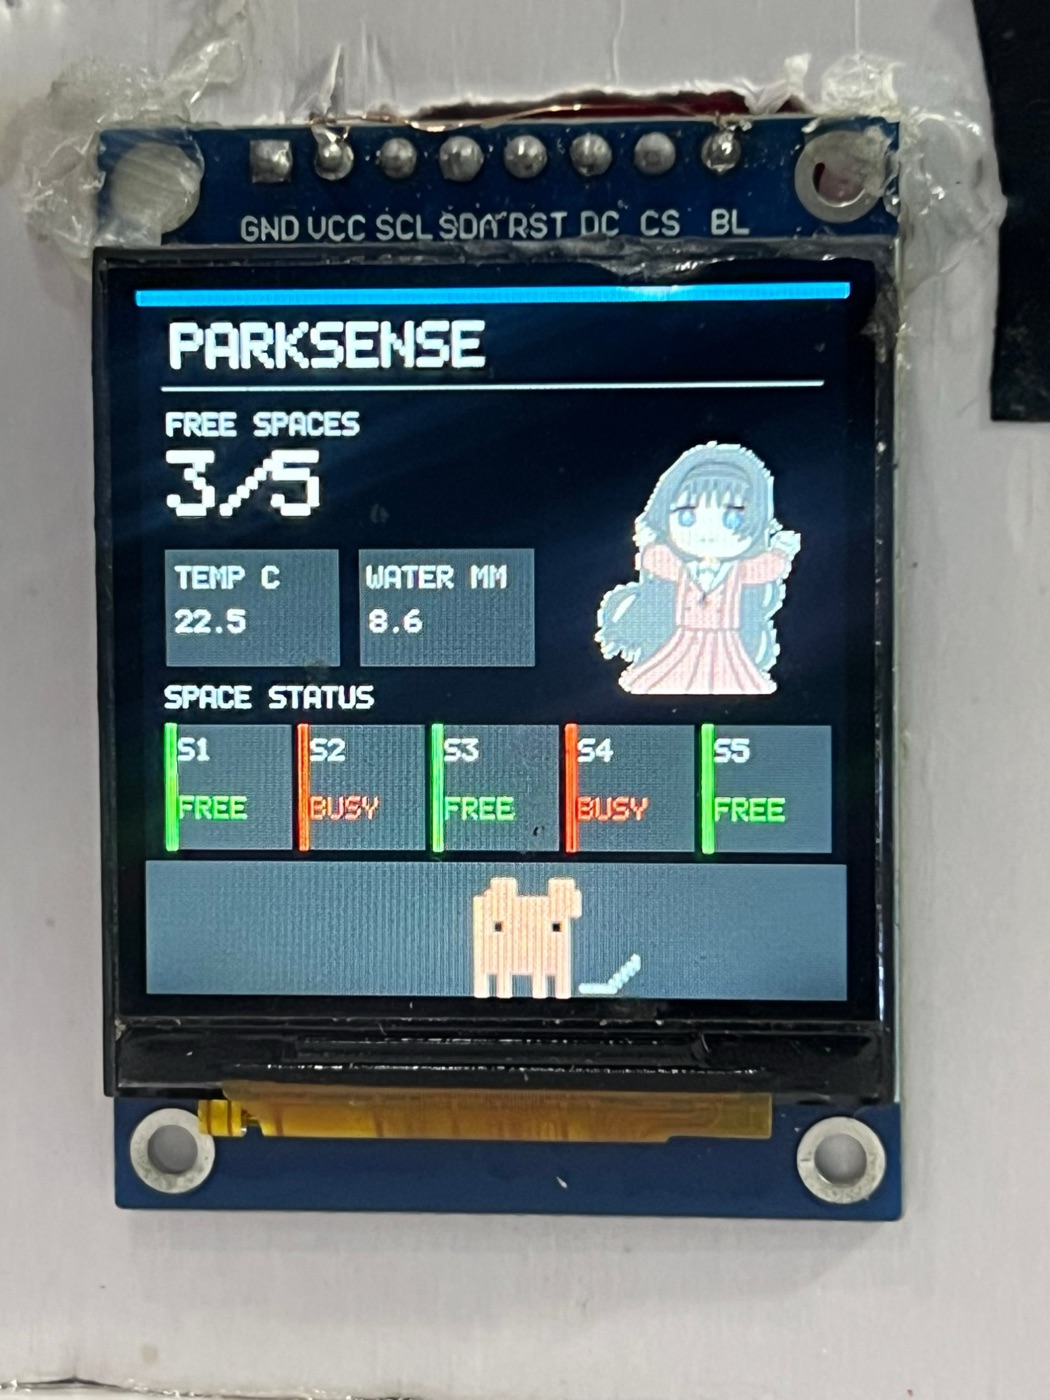
\includegraphics[width=\linewidth,height=0.3\textheight,keepaspectratio]{photos/tft_live.jpg}
  \caption{Màn hình TFT ở mặt trước hộp điều khiển}\label{fig:tft-live}
\end{subfigure}
\caption{Bố trí phần cứng trên mô hình}\label{fig:hw-photos}
\end{figure}

Hình~\ref{fig:model-back} là mặt ngoài vách sau, nơi đặt toàn bộ Sensor Client: năm module
hồng ngoại có đầu phát và thu xuyên qua lỗ khoét, hướng vào giữa từng ô; module lửa màu đỏ
nằm giữa dãy để góc nhìn khoảng 60° bao quát cả năm ô; module ESP8266, tụ lọc, hai diode và
jack nguồn nằm cùng mặt vách. Bố trí module và dây ở mặt ngoài giữ cho lòng bãi gọn và mỗi
module vẫn có biến trở để chỉnh ngưỡng theo độ phản xạ thực tế. Cảm biến mực nước đặt sát
sàn ở góc trong của vách sau, nơi nước đọng trước tiên. Hình~\ref{fig:gate-ir} là cổng ra:
module hồng ngoại gắn ngay trước trục servo, tia hồng ngoại chiếu ngang làn xe dưới cần chắn.
Hình~\ref{fig:box} là bên trong hộp điều khiển, nơi đặt máy chủ ESP32-C3, còi, RFID Client
cùng mạch nguồn của nó; hai đầu đọc RC522 gắn ở hai thành hộp, mỗi đầu đọc quay ra một làn,
và cảm biến DHT11 gắn ở mặt ngoài hộp để không đo nhầm nhiệt tỏa ra từ các module.
Hình~\ref{fig:tft-live} là màn hình ở mặt trước hộp, quay về phía người lái.

\section{Thiết kế giao thức truyền thông}\label{sec:giaothuc}
Sensor Client và RFID Client gửi ba loại bản tin JSON tới máy chủ qua UDP. Mã nguồn~\ref{lst:msg} là ví dụ
của từng loại cùng gói xác nhận mà máy chủ gửi lại.

\begin{lstlisting}[language=json,caption={Các bản tin UDP giữa client và máy chủ},label={lst:msg}]
{"type":"parking_update","slots":[1,0,0,1,0],"water_mm":0.2,"fire":false}
{"type":"climate","temperature_c":28.0}
{"type":"rfid_event","card_id":"A1B2C3D4","gate":"in","temperature_c":28.0,"seq":305441741}
{"type":"rfid_ack","seq":305441741}
\end{lstlisting}

Trong Mã nguồn~\ref{lst:msg}, bản tin \code{parking\_update} mang toàn bộ trạng thái của Sensor
Client gồm năm ô đỗ, mực nước và cờ cháy; bản tin \code{climate} mang nhiệt độ; bản tin
\code{rfid\_event} mang mã thẻ, cổng và số thứ tự \code{seq}. Vì cổng UDP là ranh giới tin
cậy mà mọi thiết bị trong mạng đều gửi tới được, máy chủ kiểm tra chặt từng bản tin bằng bộ
đọc JSON tự viết, không cấp phát bộ nhớ động và chỉ chấp nhận đúng lược đồ: mảng \code{slots}
đúng 5 phần tử 0 hoặc 1, mực nước 0--10\,000\,mm, nhiệt độ $-40$ đến 125\,°C, mã thẻ 1--31 ký
tự chữ, số, gạch nối; khóa lạ, khóa lặp hay dữ liệu thừa đều bị từ chối và trạng thái cũ được
giữ nguyên. So với thư viện cJSON, cách làm này tránh phân mảnh bộ nhớ khi chạy lâu và giới
hạn được thời gian xử lý mỗi bản tin.

Phía trang web, máy chủ cung cấp các API HTTP được liệt kê ở Bảng~\ref{tab:api}. Mọi lệnh làm
thay đổi trạng thái dùng phương thức POST và phải mang mã PIN quản trị trong header
\code{X-Parking-Key}; sai mã PIN, máy chủ trả mã lỗi 401.

\begin{table}[H]
\centering\small
\caption{API HTTP của máy chủ}\label{tab:api}
\begin{tabularx}{\linewidth}{@{}lp{6.2cm}X@{}}
\toprule
Phương thức & Đường dẫn & Chức năng \\ \midrule
GET & \code{/api/parking} & Trạng thái ô đỗ, số chỗ trống, nhiệt độ, mực nước, cháy, ngập \\
GET & \code{/api/barrier} & Trạng thái hai thanh chắn \\
GET & \code{/api/rfid} & Xe trong bãi, lượt thanh toán đang chờ, 10 sự kiện gần nhất, doanh thu \\
POST & \code{/api/barrier/<cổng>/<lệnh>} & Mở hoặc đóng cổng \code{in}, \code{out} hoặc \code{all} \\
POST & \code{/api/payment/confirm} & Người vận hành xác nhận đã nhận tiền \\
POST & \code{/api/rfid/remove} & Xóa một xe khỏi danh sách trong bãi \\
POST & \code{/api/time} & Trình duyệt cung cấp giờ thực cho máy chủ \\
\bottomrule
\end{tabularx}
\end{table}

Các API trong Bảng~\ref{tab:api} được trang web gọi theo chu kỳ 1--2\,s. Cách hỏi vòng này không
giữ trạng thái kết nối trên máy chủ, mỗi yêu cầu được xử lý xong là giải phóng, phù hợp với
giới hạn bộ nhớ và số kết nối đồng thời của vi điều khiển; độ trễ thêm tối đa một giây là chấp
nhận được với dữ liệu thay đổi theo giây.
